%!TeX root = main.tex
\chapter{DIE Klasse der Fourier-Transformationen}
In diesem Kapittel werden Beispiele einer speziellen Klasse von $\cD$-Moduln
diskutiert. Dazu wird im folgendem zu 2 Beispielen explizit der Beweis aus
\cite{sabbah_cimpa90} zur Levelt-Turrittin-Zerlegung nachvollzogen.

\section{Rezept für allgemeine $\phi$} \label{sec:allgemeinProblem}
Hier wollen wir nun eine Spezielle Klasse von Meromorphen Zusammenhängen, die
die durch das folgende Rezept entstehen.
\begin{enumerate}
\item Wähle zunächst ein $\phi$
$\in\{\phi=\sum_{k\in I}\frac{a_k}{t^{k}}|I\subset\N\mbox{ endlich}
,a_k\in \C\}$
aus
\item und beginne mit $\sE^{\phi}=\cD_{\hat L}/\cD_{\hat L}\cdot \tilde Q$
mit
$ \tilde Q(t,\partial_t):=\partial_t-\frac{d}{dt}\phi(t)$
$\in\C[t,t^{-1}]<\partial_t>$.
\item Wir wollen aber ein Element in $\C[t]<\partial_t>$,
deshalb multipliziere mit Hauptnenner und erhalte
\begin{align*}
\cD_{\hat L}\cdot \tilde Q(t,\partial_t)
  &=\cD_{\hat L}\cdot (\underset{\in\C[t]\subset\cD_{\hat L}^*}
    {\underbrace{\mbox{Hauptnenner }}}
  \cdot (\partial_t-\frac{d}{dt}\phi(t))) \\
&=\cD_{\hat L}\cdot ( \underset{=:Q(t,\partial_t)}{\underbrace{
  t^{\max(I)+1} \cdot (\partial_t-\frac{d}{dt}\phi(t))}})
  & & \vartriangleleft\cD_{\hat L}
\end{align*}
mit $Q\in\C[t]<\partial_t>$.
Dies ändert den Assozierten Meromorphen Zusammenhang nicht, weil
$t^{\max(I)+1}$ eine Einheit in $\cD_{\hat L}$ ist.
\item Fouriertransformiere $Q$ und erhalte
$\cF_Q(z,\partial_z)=Q(\partial_z,-z)$ in $\C[z]<\partial_z>$
\item Wende den Übergang $x\rightsquigarrow z^{-1}$ an.\\
Was passiert mit der Ableitung $\partial_x$? Es gilt
\[
\partial_x (f(\frac{1}{x}))=
\partial_z(f)\cdot (-\frac{1}{x^2})=
-\partial_z(f)\cdot z^2= %TODO: wegen klammerung?
- z^2 \cdot \partial_z(f)
\]
also $ \partial_x\rightsquigarrow-z^2\partial_z $.
\[
P_\phi(x,\partial_x):=\cF_Q(x^{-1},-x^2\partial_x) \in \C[t]<\partial_t>
\]
\item Erhalte den zu $P_\phi$ assoziierten Meromorphen Zusammenhang
$\cM_\phi=\cD_{\hat K}/\cD_{\hat K}\cdot P_{\phi}$.
\end{enumerate}

\begin{comment}
warum sind diese wichtig??
\end{comment}

\paragraph{Wende das Rezept allgemein für
$\phi=\sum_{k\in I}\frac{a_k}{t^{k}}$ an.}
So ist
\begin{align*}
\tilde Q(t,\partial_t) &=\partial_t-\frac{d}{dt}\phi(t) \\
                       &=\partial_t+\sum_{k\in I} k\frac{a_k}{t^{k+1}}
                       & &\in \C[t][t^{-1}]<\partial_t>\\
Q(t,\partial_t)        &=t^{\max(I)+1}\partial_t
                         +\sum_{k\in I} k\frac{a_k}{t^{k-\max(I)}} \\
                       &=t^{\max(I)+1}\partial_t
                         +\sum_{k\in I}k a_k t^{\max(I)-k}
                       & &\in \C[t]<\partial_t>\\
\cF_Q(z,\partial_z)    &=Q(\partial_z,-z)\\
                       &=-\partial_z^{\max(I)+1}z
                         +\sum_{k\in I}k a_k\partial_z^{\max(I)-k} \\
P_{\phi}(x,\partial_x) &=\cF_Q(x^{-1},-x^2\partial_x) \\
                       &=-(-x^2\partial_x)^{\max(I)+1}x^{-1}
                         +\sum_{k\in I}k a_k(-x^2\partial_x)^{\max(I)-k} \\
                       &=(-x^2\partial_x)^{\max(I)}
                         \underbracket{x^2\partial_xx^{-1}}
                         +\sum_{k\in I}k a_k(-x^2\partial_x)^{\max(I)-k} \\
%TODO; weiter ausführen, genauer, nebenrechnung
                       &=(-x^2\partial_x)^{\max(I)}
                         \overbracket{(x\partial_x-1)}
                         +\sum_{k\in I}k a_k(-x^2\partial_x)^{\max(I)-k}
                       & &\in \C[x]<\partial_x>
\end{align*}
Im Anhang \ref{chap:zu-rezept} wird das $(x^2\partial_x)^{k}$ genauer
diskutiert. Dies führt aber hier an dieser Stelle nicht mehr weiter in die
richtige Richtung.

\paragraph{Ab jetzt nur noch für den Spezialfall $\phi=\frac{a}{t^{q}}$.}
Also sei $\cM_\phi=\cD_{\hat K}/\cD_{\hat K}\cdot P_\phi$ mit
\[
P_{\phi}(x,\partial_x) =(-x^2\partial_x)^{q} (x\partial_x-1)+qa \,,
\]
so dass
\begin{lem}
$\cP(\cM_{\phi})=\{\frac{q}{q+1}\}$ gilt.
\end{lem}
\begin{proof} \cite[5.b.]{sabbah_Fourier-local}
TODO
\begin{comment}
über L-Symbol? Stützfunktion? Versuch:\\
Mit $L=q s_0 + (q+1)s_2$ gilt
\[
\sigma_L(P)= \pm x^{2q+1}\partial_x^{q+1} + qa \,,
\]
welches aus mehr als einem Monom besteht, deshalb ist der zu $L$ zugehörige
Slope $\frac{q}{q+1}$ ein Slope von $P$. Da $q+1$ die höchste vorkommende
$\partial_x$-Potez ist, kann es auch keinen weiteren Slope geben.
\end{comment}
\end{proof}
Also ist ein pull-back mit Grad $q+1$ nötig, um einen ganzzahligen Slope zu
bekommen.
Sei $\rho:t\mapsto x:=t^{q+1}$ so ist
\begin{align*}
\rho^+\cM_\phi &= \rho^+(\cD_{\hat K}/\cD_{\hat K}\cdot P_\phi(x,\partial_x))\\
  &=\cD_{\hat K}/\cD_{\hat K}\cdot(\rho^*P_\phi(x,\partial_x))\\
  &=\cD_{\hat K}/\cD_{\hat K}\cdot(P_\phi(\rho(t),\rho'(t)^{-1}\partial_t))\\
  &=\cD_{\hat K}/\cD_{\hat K}
    \cdot(P_\phi(t^{q+1},\frac{1}{(q+1)t^q}\partial_t))\\
  %&=\cD_{\hat K}/\cD_{\hat K}\cdot((-\rho(t)^2\rho'(t)^{-1}\partial_t)^{q}
    %(\rho(t)\rho'(t)^{-1}\partial_t-1)+qa)\\
  &=\cD_{\hat K}/\cD_{\hat K}
    \cdot((-(t^{q+1})^2\frac{1}{(q+1)t^{q}}\partial_t)^{q}
    (t^{q+1}\frac{1}{(q+1)t^{q}}\partial_t-1)+qa)\\
  &=\cD_{\hat K}/\cD_{\hat K}
    \cdot((-\frac{1}{q+1}t^{2(q+1)-q}\partial_t)^{q}
    (\frac{1}{q+1}t\partial_t-1)+qa)\\
  &=\cD_{\hat K}/\cD_{\hat K}
    \cdot((-\frac{1}{q+1}t^{q+2}\partial_t)^{q}
    (\frac{1}{q+1}t\partial_t-1)+qa)
\end{align*}
\begin{comment}
Sei $\rho:t\mapsto x:=-(q+1) t^{q+1}$ so ist
\begin{align*}
\rho^+\cM_\phi &= \rho^+(\cD_{\hat K}/\cD_{\hat K}\cdot P_\phi(x,\partial_x))\\
  &=\cD_{\hat K}/\cD_{\hat K}\cdot(\rho^*P_\phi(x,\partial_x))\\
  &=\cD_{\hat K}/\cD_{\hat K}\cdot(P_\phi(\rho(t),\rho'(t)^{-1}\partial_t))\\
  &=\cD_{\hat K}/\cD_{\hat K}
    \cdot(P_\phi(-(q+1) t^{q+1},-(q+1)^{-1}\frac{1}{(q+1)t^q}\partial_t))\\
  &=\cD_{\hat K}/\cD_{\hat K} \cdot
    ((-(-(q+1) t^{q+1})^2\frac{-(q+1)^{-1}}{(q+1)t^{q}}\partial_t)^{q}
    (-(q+1) t^{q+1}\frac{-(q+1)^{-1}}{(q+1)t^{q}}\partial_t-1)+qa)\\
  &=\cD_{\hat K}/\cD_{\hat K}
    \cdot((-\frac{-(q+1)}{q+1}t^{2(q+1)-q}\partial_t)^{q}
    (\frac{1}{q+1}t\partial_t-1)+qa)\\
  &=\cD_{\hat K}/\cD_{\hat K}
    \cdot((t^{q+2}\partial_t)^{q}
    (\frac{1}{q+1}t\partial_t-1)+qa)
\end{align*}
\end{comment}
mit $\cP(\rho^+\cM_\phi)=\{q\}\subset\N$. Definiere mittels
$q=\frac{q}{1}=:\frac{\lambda_0}{\lambda_1}$ die  Linearform
\[
L(s_0,s_1)=\lambda_0s_0+\lambda_1s_1=qs_0+s_1 \,.
\]
Schreibe $\rho^*P_{\phi}=\sum_i\sum_j\alpha_{ij}t^j\partial_t^i$ und berechne
die \emph{Determinanten Gleichung} $\sigma_L(\rho^*P_{\phi})\in \hat K[\xi]$.
\begin{align*}
\sigma_L(\rho^*P_{\phi})
  &= \sum_{\{(i,j)\in\N\times\Z \mid L(i,i-j)=0\}}\alpha_{ij}x^j\xi^i\\
  &= \sum_{\{(i,j)\in\N\times\Z \mid (q+1)i-j=0\}}\alpha_{ij}x^j\xi^i
\end{align*}
Da $\hat K[\xi]$ kommutativ ist gilt hier, dass $(x^j\xi^i)^k=x^{jk}\xi^{ik}$ ist.
Setze $\theta=x^{\lambda_0+\lambda_1}\xi^{\lambda_1}=x^{q+1}\xi$ so können wir
\begin{align*}
\sigma_L(\rho^*P_{\phi}) &= \sum_{k\geq 0}\alpha_k\theta^k
\end{align*}
schreiben, welches wir als nächsten Schritt faktorisieren
\[
\sigma_L(\rho^*P_\phi)=\epsilon\prod_{\beta}(\theta-\beta)^{\gamma_\beta}\,.
\]
Wobei $\epsilon\in\C$ eine Konstante ist.
Sei $\beta_0$  eine der Nullstellen.
Es ist $0$ keine Nullstelle von $\sigma_L(\rho^*P_\phi)$ da $\alpha_0\neq 0$.
Setze $R(z):=(\beta_0/(\lambda_0+1))z^{\lambda_0+1}=(\beta_0/(q+1)z^{q+1}$ und
betrachte
\begin{align*}
\rho^+\cM_\phi\otimes\cF_{\hat K}^R
  &= \cD_{\hat K}/\cD_{\hat K}\cdot(\rho^*P_{\phi})\otimes\cF_{\hat K}^R \,.
\end{align*}
\begin{lem}
Sei $e$ ein zyklischer Vektor zu $\rho^+\cM_\phi$, so ist $e\otimes e(R)$ ein
zyklischer Vektor für $\rho^+\cM_\phi\otimes\cF_{\hat K}^R$.
\end{lem}

\section{Spezialfall $\phi_1:=\frac{a}{x}$}
Das wohl einfachste Beispiel ist $\cM_{\phi_1}$ bezüglich
$\phi_1:=\frac{a}{x}$.
\begin{align*}
P_{\phi_1}(x,\partial_x) &=-x^2\partial_x (x\partial_x-1)+a \\
  &=-x^2\underbracket{\partial_xx}\partial_x+x^2\partial_x+a \\
  %&=-x(x\partial_x)^2+x(x\partial_x)+a \\
  &=-x^2\overbracket{(x\partial_x+1)}\partial_x+x^2\partial_x+a \\
  &=-x^3\partial_x^2 - x^2\partial_x+x^2\partial_x+a \\
  &=-x^3\partial_x^2+a
\end{align*}
Erhalte nun das Newton-Polygon mit den Slopes
$\cP(\cM_{\phi_1})=\{\frac{1}{2}\}$.
\begin{figure}[H]
\caption{Newton Polygon zu $P_{\phi_1}$}
\begin{center}
\fbox{
  \begin{tikzpicture}[scale=1.5,descr/.style={fill=white,inner sep=2.5pt}]
  \def\myPoints{0/0,2/1}
  \def\myPath{ -- node[descr]{$\frac{1}{2}$} (2,1)}
  \myPlotFunction{\myPoints}{\myPath}{2}{0}{1}{$N(P_{\phi_1})$}
  \end{tikzpicture}
}
\end{center}
\end{figure}
Berechne nun den pull-back mit $\rho:t\mapsto x:=t^2$
\begin{align*}
\rho^*P_{\phi_1}(x,\partial_x)
  %&=(-\frac{1}{(q+1)}t^{q+2}\partial_t)^{q}
    %(\frac{1}{(q+1)}t\partial_t-1)+qa\\
  &=-\frac{1}{2}t^{3}\partial_t
    (\frac{1}{2}t\partial_t-1)+a\\
  &=-\frac{1}{4}t^{3}\underbracket{\partial_tt}\partial_t
    +\frac{1}{2}t^{3}\partial_t+a\\
  &=-\frac{1}{4}t^{3}\overbracket{(t\partial_t+1)}\partial_t
    +\frac{1}{2}t^{3}\partial_t+a\\
  &=-\frac{1}{4}t^{4}\partial_t^2
    \underbracket{-\frac{1}{4}t^{3}\partial_t+\frac{1}{2}t^{3}\partial_t}+a\\
  &=-\frac{1}{4}t^{4}\partial_t^2
    \overbracket{+\frac{1}{4}t^{3}\partial_t}+a
\end{align*}
und erhalte einen Meromorphen Zusammenhang $\rho^+\cM_{\phi_1}=\cD_{\hat
K}/\cD_{\hat K}\cdot\rho^*P_{\phi_1}$ mit genau dem Slope
$1=\frac{1}{1}=:\frac{\lambda_0}{\lambda_1}$.
\begin{figure}[H]
\caption{Newton Polygon zu $\rho^*P_{\phi_1}$}
\begin{center}
\fbox{
  \begin{tikzpicture}[scale=1.5,descr/.style={fill=white,inner sep=2.5pt}]
  \def\myPoints{0/0,1/2,2/2}
  \def\myPath{ -- node[descr]{$1$} (2,2)}
  \myPlotFunction{\myPoints}{\myPath}{2}{0}{2}{$N(\rho^*P_{\phi_1})$}
  \end{tikzpicture}
}
\end{center}
\end{figure}
Definiere die Linearform $L(s_0,s_1):=\lambda_0s_0+\lambda_1s_1=s_0+s_1$.
Berechne nun die \emph{Determinanten Gleichung} $\sigma_L(\rho^*P_{\phi_1})\in
\hat K[\xi]$ von $\rho^*P_{\phi_1}$.
\begin{align*}
\sigma_L(\rho^*P_{\phi_1})
  &= \sum_{\{(i,j)\mid 2i-j=0\}}\alpha_{ij}x^{j}\xi^i\\
  &= -\frac{1}{4}x^4\xi^2 + a
\end{align*}
Setze $\theta:=x^{\lambda_0+\lambda_1}\xi^{\lambda_1}=x^2\xi$ so erhalten wir
\begin{align*}
\sigma_L(\rho^*P_{\phi_1}) &= -\frac{1}{4}\theta^2 + a
\end{align*}
schreiben, welches wir als nächstes faktorisieren
\begin{align*}
\sigma_L(\rho^*P_{\phi_1}) &= -\frac{1}{4}\theta^2+a\\
  &=-\frac{1}{4}(\theta^2-4a)\\
  &=-(\theta-\underset{=:\beta_0}{\underbrace{2\sqrt{a}}})(\theta+2\sqrt{a})
\end{align*}
Dies geht, weil $\hat K[\xi]$ kommutativ ist.
Setze $R(z):=(\beta_0/(\lambda_0+1))z^{\lambda_0+1}=\sqrt{a}z^2$ und betrachte
$\rho^+\cM_{\phi_1}\otimes\cF_{\hat K}^R$.
\begin{comment}
BIS HIER HIN KORREGIERT: $P_\phi$ ist im folgendem FALSCH
\end{comment}

\subsection{Sabah's refined Levelt-Turrittin-Zerlegung für $\phi_1$}

\section{Angewendet für $\phi_2:=\frac{a}{x^2}$}
\begin{comment}
für $q=2$
%
\begin{align*}
P_{\phi}(x,\partial_x) &=(-x^2\partial_x)^2 (x\partial_x-1)+2a \\
  &=x^2\underbracket{\partial_xx^2}\partial_x(x\partial_x-1)+2a \\
  &=x^2\overbracket{(x^2\partial_x+2x)}\partial_x(x\partial_x-1)+2a \\
  &=(x^4\partial_x^2+2x^3\partial_x)(x\partial_x-1)+2a \\
  &=x^4\underbracket{\partial_x^2x}\partial_x
    +2x^3\underbracket{\partial_xx}\partial_x
    -x^4\partial_x^2-2x^3\partial_x+2a \\
  &=x^4\overbracket{(x\partial_x^2+2x)}\partial_x
    +2x^3\overbracket{(x\partial_x+1)}\partial_x
    -x^4\partial_x^2-2x^3\partial_x+2a \\
  &=x^5\partial_x^3+2x^5\partial_x +2x^4\partial_x^2 +2x^3\partial_x
    -x^4\partial_x^2-2x^3\partial_x+2a \\
  &=3x^5\partial_x^3 +x^4\partial_x^2 + 2a
\end{align*}
\end{comment}

\textbf{also für $\phi_2:=\frac{a}{x^2}$} ist
\begin{align*}                                                                       !
P_{\phi_2} &=2a+x\partial_x\underbracket{(-x^2\partial_x)^{2}}\\
           &=2a +x\partial_x \overbracket{(2x^3\partial_x+x^4\partial_x^2)} \\
           &=2a
             +2x\underbracket{\partial_xx^3}\partial_x
             +x\underbracket{\partial_xx^4}\partial_x^2 \\
           &=2a
             +2x\overbracket{(3x^2+x^3\partial_x)}\partial_x
             +x\overbracket{(4x^3+x^4\partial_x)}\partial_x^2 \\
           &=2a+5x^3\partial_x+4x^{4}\partial_x^2+x^5\partial_x^3
\end{align*}
\begin{figure}[H]
\caption{Newton Polygon zu $P_{\phi_2}$}
\begin{center}
\fbox{
  \begin{tikzpicture}[scale=1.5,descr/.style={fill=white,inner sep=2.5pt}]
  \def\myPoints{0/0,1/2,2/2,3/2}
  \def\myPath{ -- node[descr]{$\frac{2}{3}$} (3,2)}
  \myPlotFunction{\myPoints}{\myPath}{3}{0}{2}{}
  \end{tikzpicture}
}
\end{center}
\end{figure}

\subsection{Levelt-Turrittin-Zerlegung für $\phi_2$}
$\cM_{\phi_2}$ hat genau den Slope $\frac{2}{3}$ mit Nenner $3$.\\
Sei $\rho:t\mapsto x:=t^3$ und betrachte
\begin{align*}
\rho^+\cM_{\phi_1} &= \rho^+\Big( \cD_{\hat K}/\cD_{\hat
  K}\cdot(2a+5x^3\partial_x+4x^{4}\partial_x^2+x^5\partial_x^3) \Big) \\
&= \cD_{\hat L}/\cD_{\hat L}\cdot(2a+
  5\rho(t)^3(\rho'(t)^{-1}\partial_t)
  +4\rho(t)^{4}(\rho'(t)^{-1}\partial_t)^2
  +\rho(t)^5(\rho'(t)^{-1}\partial_t)^3) \\
&= \cD_{\hat L}/\cD_{\hat L}\cdot(2a+
  5t^9(\frac{1}{3}t^{-2}\partial_t)
  +4t^{12}(\frac{1}{3}t^{-2}\partial_t)^2
  +t^{15}(\frac{1}{3}t^{-2}\partial_t)^3) \\
&= \cD_{\hat L}/\cD_{\hat L}\cdot(2a+
  \frac{5}{3}t^7\partial_t
  +\frac{4}{9}t^{12}(t^{-2}
    \underbracket{\partial_tt^{-2}}
    \partial_t)
  +\frac{1}{27}t^{15}(t^{-2}
    \underbracket{\partial_tt^{-2}}
    \underbracket{\partial_tt^{-2}}
    \partial_t)) \\
&\begin{aligned}
&= \cD_{\hat L}/\cD_{\hat L}\cdot(2a+
  \frac{5}{3}t^7\partial_t
  +\frac{4}{9}t^{10}
    \overbracket{(t^{-2}\partial_t-2t^{-3})}
    \partial_t\\
  &\qquad+\frac{1}{27}t^{13}
    \underbracket{
      \overbracket{(t^{-2}\partial_t-2t^{-3})}
      \overbracket{(t^{-2}\partial_t-2t^{-3})}
    }
    \partial_t) \\
\end{aligned}\\
&\begin{aligned}
&= \cD_{\hat L}/\cD_{\hat L}\cdot(2a+
  \frac{5}{3}t^7\partial_t
  +\frac{4}{9}t^{8}\partial_t^2
  -\frac{8}{9}t^{7}\partial_t\\
  &\qquad+\frac{1}{27}t^{13}
    \overbracket{(
      t^{-2}\underbracket{\partial_tt^{-2}}\partial_t
      -2t^{-2}\underbracket{\partial_tt^{-3}}
      -2t^{-5}\partial_t
      +4t^{-6}
    )}
    \partial_t) \\
\end{aligned}\\
&\begin{aligned}
  &= \cD_{\hat L}/\cD_{\hat L}\cdot(2a+
    (\frac{5}{3}-\frac{7}{9}+\frac{4}{27})t^7\partial_t
    +(\frac{4}{9}-\frac{2}{27})t^{8}\partial_t^2
    +\frac{1}{27}t^{11}\overbracket{(t^{-2}\partial_t-2t^{-3})}\partial_t^2\\
    &\qquad-\frac{2}{27}t^{11}\overbracket{(t^{-3}\partial_t-3t^{-4})}
      \partial_t
  )
\end{aligned}\\
%&\begin{aligned}
  %&= \cD_{\hat L}/\cD_{\hat L}\cdot(2a+
    %(\frac{5}{3}-\frac{7}{9}+\frac{4}{27})t^7\partial_t
    %+(\frac{4}{9}-\frac{2}{27})t^{8}\partial_t^2
    %+\frac{1}{27}t^{9}\partial_t^3-\frac{2}{27}t^{8}\partial_t^2\\
    %&\qquad -\frac{2}{27}t^{8}\partial_t^2 +\frac{6}{27}t^{7}\partial_t
  %)
%\end{aligned}\\
&= \cD_{\hat L}/\cD_{\hat L}\cdot(2a+
  \frac{28}{27}t^7\partial_t
  +\frac{10}{27}t^{8}\partial_t^2
  +\frac{1}{27}t^{9}\partial_t^3-\frac{2}{27}t^{8}\partial_t^2
  -\frac{2}{27}t^{8}\partial_t^2 +\frac{6}{27}t^{7}\partial_t
)\\
&= \cD_{\hat L}/\cD_{\hat L}\cdot(2a+ \frac{34}{27}t^7\partial_t
  +\frac{6}{27}t^{8}\partial_t^2 +\frac{1}{27}t^{9}\partial_t^3)
\end{align*}
\begin{figure}[H]
\caption{Newton Polygon zu $\rho^*P_{\phi_2}$}
\begin{center}
\fbox{
  \begin{tikzpicture}[scale=1.5,descr/.style={fill=white,inner sep=2.5pt}]
  \def\myPoints{0/0,1/6,2/6,3/6}
  \def\myPath{ -- node[descr]{$2$} (3,6)}
  \myPlotFunction{\myPoints}{\myPath}{3}{0}{6}{}
  \end{tikzpicture}
}
\end{center}
\end{figure}
Nun hat $\rho^*\cM_{\phi_2}$ nur noch den Slope
$2=\frac{2}{1}=:\frac{\lambda_0}{\lambda_1}$ und definiere damit die Linearform
$L(s_0,s_1)=\lambda_0s_0+\lambda_1s_1$.  Berechne nun die \emph{Determinanten
Gleichung} $\sigma_L(\rho^*P_{\phi_2})\in \hat
K[\xi]$ von $\rho^*P_{\phi_2}$.
\begin{align*}
\sigma_L(\rho^*P_{\phi_2})
&= \sum_{\{(i,j) \mid L(i,i-j)=\ord_L(\rho^*P_{\phi_2})\}}\alpha_{ij}x^j\xi^i\\
&= \sum_{\{(i,j) \mid 2i + i-j=0\}}\alpha_{ij}x^j\xi^i\\
&= 2a+\frac{1}{27}x^9\xi^3
\end{align*}
Setze $\theta=x^{\lambda_0+\lambda_1}\xi^{\lambda_1}=x^3\xi$ so können wir
\begin{align*}
\sigma_L(\rho^*P_{\phi_2}) &= \sum_{k\geq 0}\alpha_k\theta^k\\
&= 2a+\frac{1}{27}\theta^3
\end{align*}
%Dies geht, weil $\hat K[\xi]$ kommutativ ist.
schreiben, welches wir als nächstes faktorisieren
\begin{align*}
\sigma_L(\rho^*P_{\phi_2}) &= 2a+\frac{1}{27}\theta^3\\
&=\frac{1}{27}(\theta^3-54a)\\
&=\frac{1}{27}(\theta-?)(\theta-?)(\theta-?)\\
\end{align*}

Setze $R(z):=(\beta_0/(\lambda_0+1))z^{\lambda_0+1}=\sqrt{??}z^3$ und betrachte
$\rho^+\cM_{\phi_2}\otimes\cF_{\hat K}^R$.

\section{Angewendet für $\phi_3:=\frac{1}{x}+\frac{1}{x^2}$}
\textbf{also für $\phi_3:=\frac{1}{x}+\frac{1}{x^2}$} ist
\begin{align*}
P_{\phi_3} &=x\partial_x(-x^2\partial_x)^{\max_j(k_j)}
             +\sum_{i\in I} k_i(-x^2\partial_x)^{\max_j(k_j)-k_i}\\
           &=x\partial_x\underbracket{(x^2\partial_x)^{2}}
             +1(-x^2\partial_x)^{1}+2(-x^2\partial_x)^{0}\\
           &\overbox{=}{(\ref{eq:rezeptNeben1})}
             x\partial_x \overbracket{(2x^3\partial_x+x^4\partial_x^2)}
             -x^2\partial_x+2\\
           &=2x\underbracket{\partial_xx^3}\partial_x
             +x\underbracket{\partial_xx^4}\partial_x^2
             -x^2\partial_x+2\\
           &\overbox{=}{(\ref{eq:kommutator1})}
             \underbracket{2x\overbracket{(3x^2+x^3\partial_x)}\partial_x}
             +\underbracket{x\overbracket{(4x^3+x^4\partial_x)}\partial_x^2}
             -x^2\partial_x+2\\
           &=\overbracket{6x^3\partial_x+2x^4\partial_x^2}
             +\overbracket{4x^4\partial_x^2+x^5\partial_x^3}
             -x^2\partial_x+2\\
           &= x^5\partial_x^3+6x^4\partial_x^2+(6x^3-x^2)\partial_x+2
\end{align*}
\begin{figure}[H]
\caption{Newton Polygon zu $P_{\phi_3}$}
\begin{center}
\fbox{
  \begin{tikzpicture}[scale=1.5,descr/.style={fill=white,inner sep=2.5pt}]
  \def\myPoints{0/0,1/1,1/2,2/2,3/2}
  \def\myPath{ -- node[descr]{$\frac{2}{3}$} (3,2)}
  \myPlotFunction{\myPoints}{\myPath}{3}{0}{2}{}
  \end{tikzpicture}
}
\end{center}
\end{figure}

\section{Angewendet für $\phi_4:=\frac{1}{x^2}+\frac{1}{x^3}$}
\textbf{also für $\phi_4:=\frac{1}{x^2}+\frac{1}{x^3}$} ist
\begin{align*}
P_{\phi_4} &=x\partial_x(-x^2\partial_x)^{\max_j(k_j)}
             +\sum_{i\in I} k_i(-x^2\partial_x)^{\max_j(k_j)-k_i}\\
           &=-x\partial_x\underbracket{(x^2\partial_x)^{3}}
             -2x^2\partial_x +3\\
           &\overbox{=}{(\ref{eq:rezeptNeben1})}
             -x\partial_x\overbracket{(5x^4\partial_x+4x^{5}\partial_x^2
             +x^6\partial_x^3)}-2x^2\partial_x +3\\
           &=-5x\underbracket{\partial_xx^4}\partial_x
             -4x\underbracket{\partial_xx^{5}}\partial_x^2
             -x\underbracket{\partial_xx^6}\partial_x^3
             -2x^2\partial_x +3\\
           &\overbox{=}{(\ref{eq:kommutator1})}
             \underbracket{-5x\overbracket{(4x^3+x^4\partial_x)}\partial_x}
             \underbracket{-4x\overbracket{(5x^4+x^{5}\partial_x)}\partial_x^2}
             \underbracket{-x\overbracket{(6x^5+x^6\partial_x)}\partial_x^3}
             -2x^2\partial_x+3\\
           &=\overbracket{-20x^4\partial_x-5x^5\partial_x^2}
             \overbracket{-20x^5\partial_x^2-4x^{6}\partial_x^3}
             \overbracket{-6x^6\partial_x^3-x^7\partial_x^4}
             -2x^2\partial_x +3\\
           &=-x^7\partial_x^4-10x^6\partial_x^3-25x^5\partial_x^2
             -(20x^4+2x^2)\partial_x+3\\
\end{align*}
\begin{figure}[H]
\caption{Newton Polygon zu $P_{\phi_4}$}
\begin{center}
\fbox{
  \begin{tikzpicture}[scale=1.5,descr/.style={fill=white,inner sep=2.5pt}]
  \def\myPoints{0/0,1/1,1/3,2/3,3/3,4/3}
  \def\myPath{ -- node[descr]{$\frac{3}{4}$} (4,3)}
  \myPlotFunction{\myPoints}{\myPath}{4}{0}{3}{}
  \end{tikzpicture}
}
\end{center}
\end{figure}


% vim: set ft=tex :
